% Gerado por scripts/gerar_artigo_grafos.py a partir de
% dissertacao_frotas/resultados/logs/relatorio_analise_grafos_neo4j.json. Não editar à mão.
\section{Teste e análise do grafo persistido}
\label{sec:grafos-teste}
O grafo persistido no Neo4j foi lido de volta e submetido a três testes de consistência e a cinco análises (script scripts/analise\_grafos\_frotas.py). Os indicadores por oficina — glosa, entendida como a redução entre o valor orçado e o aprovado, e a marcação de anomalia do Isolation Forest do Capítulo 4 — foram ligados ao grafo pela mesma pseudonimização HMAC da carga, sem gravar identificadores originais.

\subsection{Testes de consistência}

Os três testes foram aprovados (Tabela~\ref{tab:grafos-testes}). A projeção entre oficinas recalculada a partir das arestas veículo–oficina coincide com a gravada em todas as 6.937 arestas, com 0 pesos divergentes. O Louvain com semente 42 sobre o grafo persistido obteve Q = 0,5650 e 19 comunidades, contra Q = 0,5646 e 18 comunidades no pipeline: a rede é a mesma, mas a ordem dos nós muda com as chaves pseudonimizadas, e o algoritmo é sensível a essa ordem.

\begin{table}[H]
\centering\small
\caption{Testes de consistência do grafo persistido}
\label{tab:grafos-testes}
\begin{tabular}{lp{0.23\textwidth}p{0.23\textwidth}p{0.23\textwidth}}
\hline
\textbf{Teste} & \textbf{Esperado} & \textbf{Observado no Neo4j} & \textbf{Resultado} \\ \hline
T1 – integridade & 7.291 veículos; 1.039 oficinas; 25.122 arestas & 7.291; 1.039; 25.122 & aprovado \\
T2 – projeção & 6.937 arestas gravadas & 6.937 recalculadas; 0 pesos divergentes & aprovado \\
T3 – reprodução & Q = 0,5646; 18 comunidades & Q = 0,5650; 19 comunidades & aprovado \\
\hline
\end{tabular}
\fonte{Elaborado pelos autores.}
\end{table}

\subsection{Significância e estabilidade das comunidades}

Algoritmos de maximização de modularidade encontram valores altos mesmo em grafos aleatórios \cite{guimera2004}. Por isso, o Q observado foi comparado com 30 redes nulas com a mesma sequência de graus, obtidas por troca dupla de arestas \cite{maslov2002}. As redes nulas atingem Q = 0,3917 $\pm$ 0,0043 (máximo de 0,4030); o valor observado, 0,5650, fica 39,9 desvios-padrão acima da média nula e supera todas as redes nulas (Figura~\ref{fig:grafos-nulo}). Em 30 sementes, Q variou de 0,5646 a 0,5651, o número de comunidades de 17 a 19, e o índice de Rand ajustado médio contra a semente 42 foi 0,983. A estrutura de comunidades é, portanto, significativa e estável, o que sustenta o resultado do pipeline original com um teste que ele não fazia.

\begin{figure}[H]
\centering
\caption{Modularidade observada contra redes nulas e concentração do gasto aprovado por oficina}
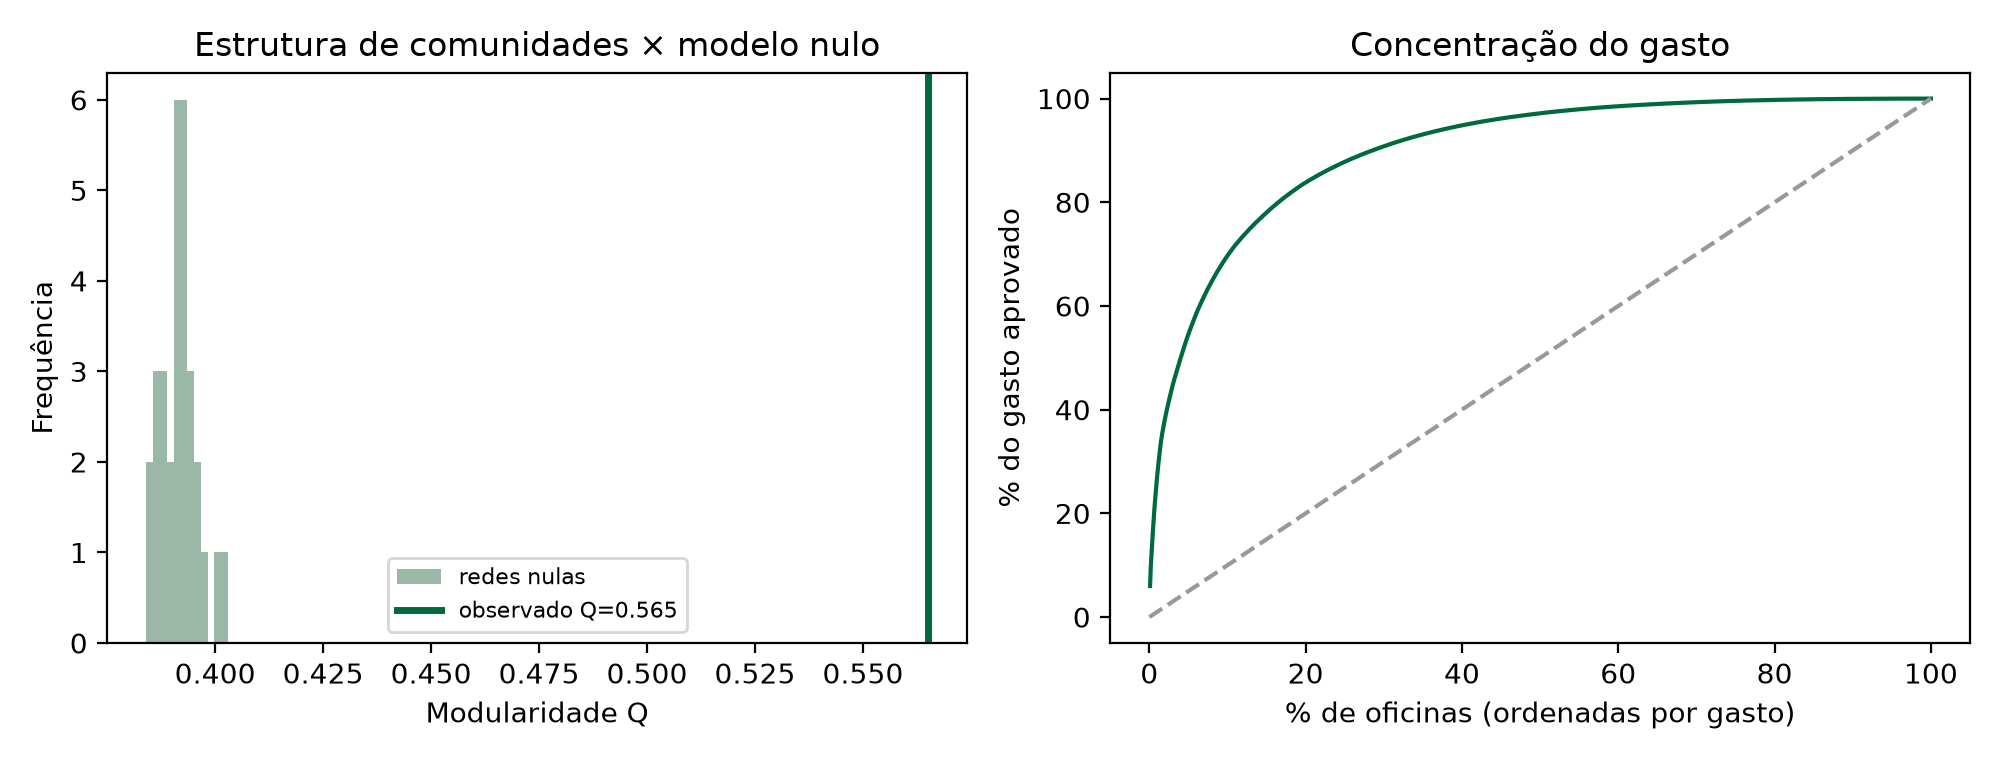
\includegraphics[width=0.95\textwidth]{figuras/grafos_modelo_nulo_e_concentracao.png}
\fonte{Dados da frota pública de Santa Catarina processados pelo autor (2026).}
\label{fig:grafos-nulo}
\end{figure}

\subsection{Indicadores de gestão derivados do grafo}

O gasto é concentrado: os 10\% de oficinas com maior gasto recebem 69,7\% do valor aprovado (Gini = 0,80). O HHI do conjunto (116 pontos) é baixo porque há mais de mil estabelecimentos, e o grafo não tem localização para medir mercados locais. Cada veículo usa, na mediana, 3 oficinas; 26,9\% usaram uma só, e a oficina principal responde, na mediana, por 68,6\% do gasto do veículo.

A Tabela~\ref{tab:grafos-spearman} relaciona a centralidade das 329 oficinas com pelo menos 30 registros aos indicadores de fiscalização. As associações são fracas: positivas com a taxa de anomalia e com a proporção glosada do orçamento, e nulas com a frequência de glosas. A taxa de glosa não difere entre as 8 maiores comunidades (Kruskal–Wallis, H = 11,66, p = 0,11).

\begin{table}[H]
\centering\small
\caption{Correlação de Spearman entre centralidade e indicadores de fiscalização (n = 329 oficinas)}
\label{tab:grafos-spearman}
\begin{tabular}{lp{0.23\textwidth}p{0.23\textwidth}p{0.23\textwidth}}
\hline
\textbf{Centralidade} & \textbf{Taxa de glosa} & \textbf{Proporção glosada do orçamento} & \textbf{Taxa de anomalia} \\ \hline
Grau ponderado & 0,088 (p 0,110) & 0,138 (p 0,012) & 0,182 (p< 0,001) \\
Intermediação & 0,097 (p 0,079) & 0,172 (p 0,002) & 0,186 (p< 0,001) \\
Veículos atendidos & 0,074 (p 0,180) & 0,160 (p 0,004) & 0,146 (p 0,008) \\
\hline
\end{tabular}
\fonte{Elaborado pelos autores. Oficinas da projeção com pelo menos 30 registros cobrados.}
\end{table}

\subsection{Implicações e limites}

O grafo é útil para descrever o mercado de manutenção e para montar amostras de auditoria por comunidade, e a centralidade pode ser um critério auxiliar de priorização. Ele não identifica irregularidades por si só: agrupamentos densos não diferem quanto a glosas, e a associação com a centralidade pode refletir o fato de oficinas maiores receberem mais ordens e mais revisão. A análise usa apenas registros cobrados, agrega todo o período, não tem localização das oficinas e aproxima a intermediação por amostragem de 400 pivôs. A comparação com o método de Leiden \cite{traag2019} fica como trabalho futuro. Esses resultados são o objeto do artigo SBC/artigo5\_grafos\_gestao\_frotas\_sbc.tex.
